We have considered so far two general methods for the computation of transport coefficients. The Green-Kubo method, which relies on analysis of autocorrelations in the fluctuation of zero-average equilibrium quantities, 
and the NEMD method, which relies in measuring the ratio in the average of a given equilibrium-centered response observable under a driven steady-state and the magnitude of the driving force.
In the case of mobility, we apply a small constant force, and measure the resulting particle flux in the direction of the perturbation. We can thus think of the mobility $\rho_F$ as measuring how \textit{responsive} the flux is to the forcing on the system.
A natural question to ask is whether it is possible to measure the dual quantity, that is, how \textit{resistive} the system is to a given flux. One possible strategy to answer this question, in loose terms, would be to \textit{constrain} the response to be constant, and measure the average magnitude of the forcing needed to maintain it.
In the limit of a small response, the linear dependency between these quantities can be hoped to provide an equivalent and reciprocal measure of the transport coefficient. By analogy with the Thévenin and Norton circuit theorems, we will from now on refer to the standard, constant-forcing method as the Thévenin method,
and the dual, constant-response method as the Norton method. We will again be using the mobility and the shear viscosity as our examples, so as to leverage our previous calculations as ways to validate our method.


\section{General framework}
We first express the method in full generality, before specializing to the non-equilibrium molecular dynamics context. We consider the stochastic differential equation:
\begin{equation}
    \label{eq:norton_general_sde}
    \left\{\begin{aligned}
        \dif X_t &= b(X_t)\,\dif t +\sigma(X_t)\,\dif W_t + \dif \Lambda_t F(X_t)\\
        R(X_t)&= r,
    \end{aligned}\right.
\end{equation}
where $b ,\sigma$ and $F$ are respectively $R^D,\, \R^{D\times E}$ and $\R^D$-valued functions, and $W$ is a $E$-dimensional Brownian motion.
We interpret $F$ as a perturbation direction for an \textit{equilibrium SDE}, and $\Lambda$ is the perturbation intensity, which is determined in order to maintain the response observable $R$ constant equal to $r>0$ along the dynamic's trajectories.
The Norton dynamics \eqref{eq:norton_general_sde} should be thought of as the constant-response counterpart to a corresponding Thévenin dynamics
\begin{equation}
        \label{eq:thevenin_general_sde}
    \left\{\begin{aligned}
        \dif X_t &= b(X_t)\,\dif t +\sigma(X_t)\,\dif W_t + \eta F(X_t),\\
        \eta>0,
    \end{aligned}\right.
\end{equation}
which is perturbed in the same direction, but with a constant forcing intensity $\eta$. Both these dynamics have a corresponding reference dynamics, respectively for $r=0$ and $\eta=0$,
with the reference Thévenin dynamics simply being the equilibrium Langevin dynamics.
For notational simplicity, let us introduce the following definitions:
\begin{equation}
    \label{eq:norton_notation}
    b_t = b(X_t),\qquad \sigma_t = \sigma(X_t),\qquad F_t= F(X_t),\qquad \nabla R_t=\nabla R(X_t),\qquad \nabla^2 R_t = \nabla^2 R(X_t).
\end{equation}
For $A,B\in\R^{D}$, such that $A\cdot B\neq 0$, we denote by $P_{A,B}$ the projector onto $A$ orthogonally to $B$
\begin{equation}
    \label{eq:non_orthogonal_projector}
    P_{A,B}=\frac{A\otimes B}{A\cdot B}.
\end{equation}
Finally, for any projector $P$, we denote by $\overline{P}$ the complementary projector
\begin{equation}
    \label{eq:complementary_projector}
    \overline{P}=\Id-P,
\end{equation}
We can now state the following result, which follows by a simple application of Itô calculus, and gives an expression for the dynamics \eqref{eq:norton_general_sde} without reference to $\Lambda$.
\begin{prop}\label{prop:norton_sde}
   Provided it is well-posed, the solution of the following SDE solves \eqref{eq:norton_general_sde}
    \begin{equation}
        \label{eq:norton_general_sde_solved}
        \dif X_t = \overline{P}_{F_t,\nabla R_t}\left[b_t\,\dif t + \sigma_t\,\dif W_t\right] - \frac{1}{2}\frac{\nabla^2 R_t : \left(\overline{P}_{F_t,\nabla R_t}\sigma_t \sigma_t^\intercal\overline{P}_{\nabla R_t,F_t}\right)}{F_t\cdot \nabla R_t}F_t\,\dif t,
    \end{equation}
    with $\Lambda_t$ taken to be an Itô process defined by
    \begin{equation}
        \label{eq:norton_sde_multiplier_solved}
        \dif \Lambda_t = -\frac{\nabla R_t \cdot b_t}{F_t\cdot \nabla R_t}\,\dif t-\frac{\nabla R_t\cdot \sigma_t\,\dif W_t}{F_t\cdot \nabla R_t}-\frac12\frac{\nabla^2 R_t : \left(\overline{P}_{F_t,\nabla R_t}\sigma_t\sigma_t^\intercal\overline{P}_{\nabla R_t,F_t}\right)}{F_t\cdot \nabla R_t}.
    \end{equation}
\end{prop}
\begin{proof}
The proof follows by analysis-synthesis.
We first assume that $\Lambda$ admits a decomposition as an Itô process,
\begin{equation}
    \label{eq:norton_multiplier_decomposition}
    \dif \Lambda_t = \lambda_t \dif t + \dif \widetilde{\Lambda}_t,
\end{equation}
where $\lambda$ is a bounded variation process and $\widetilde{\Lambda}$ is a martingale, and that $R$ sufficiently regular (say $C^2$ and bounded).
We can apply Itô's formula to the constant response condition, to get
\begin{equation}
    \label{eq:constant_response_condition}
     \nabla R_t \cdot \dif X_t + \frac12\nabla^2 R_t:\left\langle\sigma_t\,\dif W_t + \dif\widetilde{\Lambda}_tF_t\right\rangle=0,
\end{equation}
where the brackets denote the quadratic covariation of an Itô process. By identifying the martingale and bounded variation parts of the above process with $0$, we deduce an SDE for $\Lambda_t$:
\begin{equation}
    \label{eq:norton_multiplier_sde}
    \left\{\begin{aligned}
        &\nabla R_t \cdot \left( \sigma_t\,\dif W_t + F_t\,\dif \widetilde{\Lambda}_t\right)=0\\
        &\nabla R_t \cdot \left( b_t + \lambda_t F_t\right)+\frac12\nabla^2 R_t: \left\langle\sigma_t\,\dif W_t + \dif\widetilde{\Lambda}_tF_t\right\rangle=0.
    \end{aligned}\right.
\end{equation}
From the first equation, we deduce the expression of the martingale part of the forcing:
\begin{equation}
    \label{eq:norton_multiplier_martingale}
    \dif \widetilde{\Lambda}_t = - \frac{\nabla R_t\cdot \sigma_t\,\dif W_t}{\nabla R_t\cdot F_t},
\end{equation}
and as a consequence, we may compute the quadratic covariation bracket in \eqref{eq:constant_response_condition},
\begin{equation}
    \label{eq:constant_response_condition_bracket_solved}
    \left\langle\sigma_t\,\dif W_t + \dif\widetilde{\Lambda}_tF_t\right\rangle=\left\langle\left(\Id-\frac{F_t\otimes \nabla R_t}{F_t\cdot \nabla R_t}\right)\sigma_t\,\dif W_t\right\rangle = \overline{P}_{F,_t\nabla R_t}\sigma_t\sigma_t^\intercal\overline{P}^\intercal_{F_t,\nabla R_t}\,\dif t,
\end{equation}
where we use $P^\intercal_{A,B}=P_{B,A}$. Inserting equation \eqref{eq:constant_response_condition_bracket_solved} into \eqref{eq:norton_multiplier_sde} yields the full SDE for the forcing $\Lambda_t$ \eqref{eq:norton_sde_multiplier_solved} and the result follows by inserting the latter in \eqref{eq:norton_general_sde}.
\end{proof}

As stated above, we propose the Norton dynamics as a possible and alternative means of computing the linear response to a small perturbation of the equilibrium dynamics. 
We finish this general introduction by evoking a few theoretical questions related to these dynamics.
\begin{enumerate}[(i)]
    \item Existence of a unique steady-state for the dynamics \eqref{eq:norton_general_sde} and \eqref{eq:thevenin_general_sde}. As mentioned in the previous chapter, some results already exist in the Thévenin case.
    \item As before, proving the convergence of trajectory averages.
    \item With respect to the steady states, whose corresponding expectations we denote by $\E_\eta$ in the Thévenin case, and $\E_r$ in the Norton case, equality of the transport coefficients \[\underset{\eta \to 0}{\lim}\frac{\E_\eta[R]}{\eta}\] and \[\underset{r\to 0}{\lim}\frac{r}{\E_r[\lambda]}.\] This is the question of equivalence of the linear responses.
    \item Another natural question is that of the equivalence of the Norton and Thévenin equilibrium ensembles. This question asks about the existence of an asymptotic regime, or thermodynamic limit as $D\to\infty$, for which averages under the two equilibrium steady-states converge to a common value, for a sufficiently rich class of observables.
    \item On a related note, investigating the equivalence of the non-linear responses, that is the existence of a well-defined $r(\eta)$ such that the graphs $(\eta,\E_\eta[R])$ and $(\E_{r(\eta)}[\lambda],r(\eta))$ either agree or converge to a common value in some asymptotic regime when $D\to\infty$.
    \item Even more ambitiously, full equivalence of the non-equilibrium ensembles.
    \item Finally, we mention the question of finding a relation between the Norton equilibrium fluctuations of $\lambda$ and the linear response, in an analogy with the Green-Kubo formula.
\end{enumerate}
Let us mention that the question of the equivalence of of non-equilibrium ensembles has already been investigated by Evans in \cite{E93}, although the setting is purely deterministic, and the proof is formal.
The purpose of this chapter is to make somewhat rigorous a setting in which these questions are susceptible to find an answer, albeit a probably a difficult one to obtain.
Furthermore, the numerical results which we present in the remainder of this report show that these questions do not have obviously negative answers, and thus should be worthy of investigation.

\section{Norton dynamics for transport coefficients}
We now turn to specialising the setting to the Norton counterpart of the dynamics \eqref{eq:general_nemd_dynamics}. It reads
\begin{equation}
    \label{eq:norton_dynamics_general}
    \left\{ 
        \begin{aligned}
            &\dif q_t=m^{-1}p_t\,\dif t,\\
            &\dif p_t=-\nabla V(q_t)\,\dif t-\gamma M^{-1}p_t\,\dif t +\sqrt{\frac{2\gamma}\beta}\,\dif W_t +\dif \Lambda_t F(q_t),\\
            &R(q_t,p_t)=r,
        \end{aligned}
    \right.
\end{equation}
where $\Lambda_t$ is the magnitude of the perturbation, which is defined by the constraint $R(q_t,p_t)=r>0$.
We may assume $\gamma$ is a positive semi-definite diagonal matrix, as in the Thévenin case. $R$ is the response observable, which we take of the form
\[R(q,p)=G(q)\cdot p,\]
with $G$ a smooth vector field. Note in particular that $\nabla_p R(q,p)=G(q)$, and $\nabla_p^2 R(q,p)=0$. Finally note that the forcing acts solely on the momenta.
A SDE for $\Lambda_t$ can be obtained by applying Proposition \ref{prop:norton_sde}.
It immediately implies 
\begin{equation}
    \label{eq:norton_dynamics_general_solved}
    \left\{
        \begin{aligned}
            \dif q_t &= M^{-1}p_t \,\dif t\\
            \dif p_t &= \overline{P}_{F_t,G_t}\left[-\nabla V(q_t)-\dif t\gamma M^{-1}p_t\,\dif t + \sqrt{\frac{2\gamma}{\beta}}\,\dif W_t\right] - \frac{\nabla_q R_t\cdot M^{-1}p_t}{F_t\cdot G_t}F_t\,\dif t,
        \end{aligned}\right.
\end{equation}
with an expression for the forcing term
\begin{equation}
    \label{eq:norton_forcing_term}
    \left\{\begin{aligned}
        \dif \Lambda_t &= \lambda_t \,\dif t + \dif\widetilde{\Lambda}_t,\\
        \lambda_t &= \frac{G_t\cdot\left[\nabla V(q_t) + \gamma M^{-1}p_t \right] - \nabla_q R_t\cdot M^{-1}p_t}{F_t\cdot G_t},\\
        \dif \Lambda_t &= -\frac{G_t\cdot\sqrt{\frac{2\gamma}\beta}\,\dif W_t}{F_t\cdot G_t}.
    \end{aligned}\right.
\end{equation}

We use notations identical to \eqref{eq:non_orthogonal_projector}, \eqref{eq:complementary_projector} and \eqref{eq:norton_notation} in the expressions above. The bounded and martingale parts of the forcing term can be identified in \eqref{eq:norton_forcing_term}, and are given respectively by $\lambda_t$ and $\widetilde{\Lambda}_t$. 
We record the infinitesimal generator of the dynamics \eqref{eq:norton_dynamics_general_solved}, which is given by

\begin{equation}
    \label{eq:norton_general_generator}
    \cL_{\gamma}^{\mathrm{Norton}}\varphi = A \varphi - \left[\overline{P}_{F,G}\left(\nabla V+\gamma M^{-1}p\right)\right] \cdot \nabla_p\varphi - \frac{\nabla_q R \cdot M^{-1}p}{F\cdot G} F\cdot \nabla_p \varphi + \frac1\beta\nabla^2_p\varphi : \left[\overline{P}_{F,G}\gamma\overline{P}_{G,F}\right].
\end{equation}
Note $\overline{P}_{F,G}$ is a function of the coordinate variable in the equation above, and $A$ is as in \eqref{eq:Lham_splitting}.
\begin{remark}
    \label{rem:norton_sv_well_posedness}
    Note that the $G(q_t)\cdot F(q_t)$ term in the denominator may pose a question of well-posedness of the dynamics. Let us always suppose in our computations that $G(q_t)\cdot F(q_t)>0$, but this is by no means automatic.
    Indeed, thinking of the extreme case when $F$ and $G$ are orthogonal everywhere and $V=0$ highlights the fact that this is an issue of controlability: in that case, by isotropy, the component of the momentum in the direction $G$ will diffuse according to an Ornstein-Uhlenbeck process independent from any forcing applied in the direction $F$. In this case there is no way to control the response, and thus the dynamics is ill-defined. 
\end{remark}

Writing the Norton dynamics under the form \eqref{eq:norton_dynamics_general_solved} is instructive, since its structure appears clearly: its stochastic increments are comprised of the projected increments of an equilibrium Langevin dynamics, 
with an additional term involving $\nabla_q R$, which can be interpreted as a correction term enforcing the constant response constraint, in reaction to the configurational dynamics.
This fact will become clearer in the following section, where we describe splitting schemes for the Norton dynamics.

\subsection{Splitting schemes for numerical integration}
As in every case we considered so far, we will again rely on the fact that the Norton dynamics \eqref{eq:norton_dynamics_general_solved} can be split into three simpler, structure-preserving dynamics, to construct a variety of numerical schemes.
\begin{definition}[Splitting of the Norton dynamics]
    Consider the following dynamics
    \begin{equation}
        \label{eq:norton_A_dynamics}
        \left\{
            \begin{aligned}
                \dif q_t &=M^{-1}p_t\,\dif_t\\
                \dif p_t &= -\frac{\nabla_q R(q_t,p_t)\cdot M^{-1}p_t}{F(q_t)\cdot G(q_t)}F(q_t)\,\dif t
            \end{aligned}
        \right.,
    \end{equation}

    \begin{equation}
        \label{eq:norton_B_dynamics}
        \left\{
            \begin{aligned}
                \dif q_t &= 0\\
                \dif p_t &= -\overline{P}_{F_t,G_t}\nabla V(q_t)\,\dif t
            \end{aligned}
        \right.,
    \end{equation}
    and finally
    \begin{equation}
        \label{eq:norton_O_dynamics}
        \left\{
            \begin{aligned}
                \dif q_t &= 0\\
                \dif p_t &= \overline{P}_{F_t,G_t}\left[\gamma M^{-1}p_t\,\dif t +\sqrt{\frac{2\gamma}\beta}\,\dif W_t\right],
            \end{aligned}
        \right.
    \end{equation}
    which additively combine to form the Norton dynamics \eqref{eq:norton_general_sde_solved}. By analogy with the equilibrium setting, we will respectively refer to \eqref{eq:norton_A_dynamics}, \eqref{eq:norton_B_dynamics} and \eqref{eq:norton_O_dynamics} as the (Norton) $A$,$B$ and $O$ dynamics.
    At the level of the generator \eqref{eq:norton_general_generator}, this corresponds to a splitting into three operators,
    \[\cL_\gamma^{\mathrm{Norton}}=\cL_{A}^{\mathrm{Norton}}+\cL_{B}^{\mathrm{Norton}}+\cL_{\gamma,O}^{\mathrm{Norton}},\]
    with
    \begin{equation}
        \label{eq:norton_generator_splitting}
        \left\{
            \begin{aligned}
                \cL_{A}^{\mathrm{Norton}}\varphi &= A\varphi -\frac{\nabla_q R\cdot M^{-1}p}{F\cdot G}F\cdot \nabla_p \varphi,\\
                \cL_{B}^{\mathrm{Norton}}\varphi &= -(\overline{P}_{F,G}\nabla V)\cdot \nabla_p \varphi,\\
                \cL_{\gamma,O}^{\mathrm{Norton}}\varphi &= -(\overline{P}_{F,G}\gamma M^{-1}p)\cdot \nabla_p+\frac1\beta \left(\overline{P}_{F,G}\gamma\overline{P}_{G,F}\right):\nabla_p^2\varphi.
            \end{aligned}
        \right.
    \end{equation}
\end{definition}

The claim that these dynamics are structure-preserving is summed up in the following straightforward result.
\begin{lemma}
    Let $(q_t,p_t)$ refer to the solution of any of the Norton $A$,$B$ or $O$ dynamics. Then if $R(q_0,p_0)=r$, $R(q_t,p_t)=r$ for all $t>0$.
\end{lemma}
\begin{proof}
    The result can be proven by three thoughtless applications of the chain rule or Itô's formula.
    A quicker and more instructive proof follows from observing that for any $X,q,p\in \R^{dN}$, 
    \begin{align*}
        G(q) \cdot \overline{P}_{F(q),G(q)} X &= \overline{P}_{F(q),G(q)}^{\intercal}G(q)\cdot X\\
        &=\overline{P}_{G(q),F(q)}G(q)\cdot X\\
        &=0,
    \end{align*}
    since $P_{G(q),F(q)}$ is a projector onto the one-dimensional subspace spanned by $G(q)$ and $\overline{P}_{G(q),F(q)}$ is its complement. Hence any dynamics of the form 
    \[\dif q_t =0,\qquad \dif p_t = \overline{P}_{G_t,F_t}\left[b(q_t,p_t)\,\dif t +\sigma(q_t,p_t)\,\dif W_t\right]\]
    preserves $R(q_t,p_t)=G(q_t)\cdot p_t$, by applying the Itô formula, since $\nabla_p R(q,p)=G(q)$ and $\nabla_p^2 R=0$.
    This implies the result for the $B$ and $O$ dynamics. However, since the Norton dynamics also preserves $R(q_t,p_t)$ by construction, 
    the preservation property for the $A$ dynamics follows immediately, from the response conservation property of the Norton dynamics in the case $V=0$ and $\gamma=0$.
    For the more skeptical reader, we write, with $(q_t,p_t)$ a solution to the $A$ dynamics,
    \begin{align*}
        \frac{\dif}{\dif t} R(q_t,p_t) &= \nabla_q R(q_t,p_t)\cdot (M^{-1}p_t) -\nabla_p R(q_t,p_t)\cdot \left(\frac{\nabla_q R(q_t,p_t)\cdot M^{-1}p_t}{F(q_t)\cdot G(q_t)}F(q_t)\right)\\
        &= \nabla_q R(q_t,p_t)\cdot (M^{-1}p_t)\left(1-\frac{G(q_t)\cdot F(q_t)}{F(q_t)\cdot G(q_t)}\right)\\
        &=0
    \end{align*}
\end{proof}

As before, this splitting allows us to define a variety of numerical schemes for the Norton dynamics, following the same strategy as in Section \ref{section:splitting_schemes_langevin}.
In order to do so, we must prescribe a way to integrate each of the A,B and O steps individually. This is what we now turn to.
In the following, let us fix a timestep $\Dt>0$, and a response intensity $r>0$. Similar to the equilibrium setting, the B step can be integrated analytically, since its trajectories are ballistic.
Thus we have the following algorithm.
\begin{algorithm}[Norton B step]
    \begin{equation}
        \label{eq:norton_B_step}
        \left\{\begin{aligned}
            \widetilde{p}^{1} &= p^0 - \nabla V(q^0)\\
            p^{1} &= \widetilde{p}^{1} +\Dt \lambda^{1} F(q^0),
        \end{aligned}\right.
    \end{equation}
    where $\lambda^{1}$ is determined in order to conserve the response:
    \begin{equation}
        \label{eq:norton_B_step_lambda}
        G(q^0)\cdot p^{1} = r \iff \Dt\lambda^{1} = \frac{r-G(q^0)\cdot \widetilde{p}^{1}}{F(q^0)\cdot G(q^0)}.
    \end{equation}
\end{algorithm}
We next rely on the fact that the Norton O dynamics is in Ornstein--Uhlenbeck form to compute its exact solution over one timestep, using the following result.
\begin{prop}
    \label{prop:projected_ou_process}
    We consider the following general form of the Norton Ornstein--Uhlenbeck process in $\R^{dN}$. 
    \begin{equation}
        \label{eq:projected_ou_process}
        \dif p_t = - P \gamma M^{-1} p_t \,\dif t + P\sqrt{\frac{2\gamma}\beta}\,\dif W_t,
    \end{equation}  
    where $P^2=P$ is a projector (not necessarily orthogonal), $\gamma$ and $M^{-1}$ are positive definite symmetric matrices, and $W$ is a standard Brownian motion. We denote by $\overline P$ the complementary projector 
    $\overline P=\Id - P$. Assume also that $P$ and  $\gamma M^{-1}$ commute. Then, the analytical solution of \eqref{eq:projected_ou_process} writes
    \begin{equation}
        \label{eq:projected_ou_process_solved}
        p_t=\overline{P}p_0 + Pp_t^{\mathrm{eq}},
    \end{equation}
    where $p_t^{\mathrm{eq}}$ is the solution of the coupled equilibrium Ornstein--Uhlenbeck process,
    \begin{equation}
        \left\{\begin{aligned}
            \dif p_t^{\mathrm{eq}} &= - \gamma M^{-1} p_t^{\mathrm{eq}} \,\dif t + \sqrt{\frac{2\gamma}\beta}\,\dif W_t,\\
            p_0^{\mathrm{eq}} &= p_0.   
        \end{aligned}\right.
    \end{equation}
\end{prop}
\begin{proof}
    The proof follows the standard strategy of applying Itô's formula to the process rescaled by $\e^{tP\gamma M^{-1}}$. It yields
    \begin{equation}
        \dif \left(\e^{tP\gamma M^{-1}} p_t\right)=\e^{tP\gamma M^{-1}}\left(P\gamma M^{-1} p_t\,\dif t - P\gamma M^{-1}p_t \,\dif t+ P\sqrt{\frac{2\gamma}{\beta}}\,\dif W_t\right),
    \end{equation}
    whence, integrating in $t$ and multiplying both sides by $\e^{-tP\gamma M^{-1}}$,
    \begin{equation}
        p_t = \e^{-tP\gamma M^{-1}}p_0 +\int_0^t \e^{-P\gamma M^{-1}(t-s)}P\sqrt{\frac{2\gamma}{\beta}}\,\dif W_s.
    \end{equation}
    This yields an expression for the solution whatever the particular properties of $\gamma$, $M^{-1}$ and $P$. However, since $P$ is a projector, we can make use of the following useful formula: if $A$ and $P$ are square matrices with $AP=PA$, 
    \begin{equation}
        \label{eq:rodrigue_formula}
        \e^{PA}=\sum_{k=0}^\infty \frac{(PA)^k}{k!}=\sum_{k=0}^\infty \frac{P^kA^k}{k!}=\Id + P\sum_{k=1}^\infty \frac{A^k}{k!}=\Id + P\left(\e^A -\Id\right)= \overline{P}+P\e^A.
    \end{equation}
    The second equality follows from the fact that $A$ and $P$ commute, while the third follows from a repeated application of the projector identity $P=P^2=P^3=\dots$. This is sometimes referred to as Rodrigue's formula (see for instance \cite{LM15}{chapter 8}).
    Applying's Rodrigue's formula to our analytical form yields
    \begin{equation}
        p_t = \overline{P}p_0 +P\e^{-t\gamma M^{-1}}p_0 +\int_0^t \left(\overline{P}+ Pe^{-\gamma M^{-1}(t-s)}\right)P\sqrt{\frac{2\gamma}{\beta}}\,\dif W_s.
    \end{equation}
    expanding the product inside the integral, and using $\overline P P=0$, we get 
    \begin{equation}
        p_t = \overline{P}p_0 +P\e^{-t\gamma M^{-1}}p_0 +\int_0^t Pe^{-\gamma M^{-1}(t-s)}P\sqrt{\frac{2\gamma}{\beta}}\,\dif W_s.
    \end{equation}
    By our commutativity assumption, we can factor out the $P$s from the integral sign  and obtain
    \begin{equation}
        p_t = \overline{P}p_0 +P\e^{-t\gamma M^{-1}}p_0 +P^2\int_0^t e^{-\gamma M^{-1}(t-s)}\sqrt{\frac{2\gamma}{\beta}}\,\dif W_s= \overline{P}p_0 +P\left(\e^{-t\gamma M^{-1}}p_0 +\int_0^t e^{-\gamma M^{-1}(t-s)}\sqrt{\frac{2\gamma}{\beta}}\,\dif W_s\right),
    \end{equation} 
    regrouping the terms in $P$ and using again $P^2=P$. The result follows by simply recognizing the parenthesized term as $p_t^{\mathrm{eq}}$.
\end{proof}
\begin{remark}
    The commutativity assumption may seem overly restrictive, but in fact it is enough in the cases we consider. 
    For instance, in the case of shear viscosity computations with anisotropic friction, $M$ is a scalar multiple of the identity and $\gamma$ is diagonal and constant with respect to longitudinal coordinates, so that the commutativity condition is indeed verified.
\end{remark}

As a consequence of this computation, we may define a numerical strategy to integrate the fluctuation-dissipation part of the Norton dynamics.

\begin{algorithm}[Norton O step]
    \begin{equation}
        \label{eq:norton_O_step}
        \left\{
            \begin{aligned}
                \widetilde{p}^{1} &= \alpha_{\Dt}p^0 +\sigma_{\Dt}\mathcal G^1,\\
                p^{1} &= \widetilde{p}^{1} + \Dt\lambda^{1} F(q^{0}),
            \end{aligned}
        \right.
    \end{equation}
    where $\mathcal G^1$ is a standard $dN$-dimensional Gaussian, $\alpha_\Dt,\,\sigma_\Dt $ are given by \eqref{eq:alpha_sigma}, and $\lambda^{1}$ is again determined by equation \eqref{eq:norton_B_step_lambda} in order to conserve the response.
\end{algorithm}

Unfortunately, the A dynamics \eqref{eq:norton_A_dynamics} cannot be solved analytically. 
However, its general form is that of an infinitesimal Hamiltonian increment on the position coordinate, with an additional correction term in the direction $F$ on the momentum coordinate. 
Furthermore, we know the response is conserved by the A dynamics. This naturally suggests the following scheme.

\begin{algorithm}[Norton A step]
    \begin{equation}
        \label{eq:norton_A_step}
        \left\{\begin{aligned}
            q^1 &= q^0 + \Dt M^{-1}p^0, \\
            p^1 &= p^0 +\Dt\lambda^{1} F(q^1),
        \end{aligned}\right.
    \end{equation}
where $\lambda^{1}$ is determined by 
\begin{equation}
    \label{eq:norton_A_step_lambda}
    G(q^1)\cdot p^{1} = r \iff \Dt\lambda^{1} = \frac{r-G(q^1)\cdot p^0}{F(q^1)\cdot G(q^1)}
\end{equation}
to enforce the constant response constraint.
\end{algorithm}

An advantage of schemes for the Norton dynamics formed by chaining and iterating steps of \eqref{eq:norton_A_step}, \eqref{eq:norton_B_step} and \eqref{eq:norton_O_step} 
is that they immediately yield a discretization of the forcing intensity $\dif\Lambda_t$, and thus an estimation of the average $\E_r[\lambda]$, which is the quantity of prime interest to us.
Indeed, observe from equation \eqref{eq:norton_forcing_term} that we can write
\begin{equation}
    \label{eq:norton_forcing_splitting}
    \dif \Lambda_t = \lambda^{\mathrm{A}}_t \dif t + \lambda^{\mathrm{B}}_t\,\dif t + \dif \Lambda_t^{\mathrm{O}},
\end{equation}
with 
\begin{equation}
    \label{eq:norton_forcing_splitting_details}
    \left\{
    \begin{aligned}
        \lambda^{\mathrm{A}}_t &= -\frac{\nabla_q R(q_t,p_t)\cdot G(q_t)}{F(q_t)\cdot G(q_t)},\\
        \lambda^{\mathrm{B}}_t &= -\frac{\nabla V(q_t)\cdot G(q_t)}{F(q_t)\cdot G(q_t)},\\
        \dif \Lambda_t^{\mathrm{O}} &= -\frac{\left[-\gamma M^{-1}p_t\,\dif t +\sqrt{\frac{2\gamma}\beta}\,\dif W_t \right]\cdot G(q_t)}{F(q_t)\cdot G(q_t)}.
    \end{aligned}
    \right.
\end{equation}
These individual parts can be interpreted individually as the forcing intensities in the direction $F(q_t)$ applied to each of the A,B and O dynamics, relative to the corresponding equilibrium dynamics.
This yields a natural interpretation of the $\lambda^n$ terms along numerical trajectories, as discretizations of \eqref{eq:norton_forcing_splitting_details}, 
and thus one can use these ergodic averages for the average forcing. As a full example, we record the BABO-like scheme we used in our simulations, as well as the corresponding estimator of $\E_r[\lambda]$.
This procedure can of course be generalized to other orderings of the operators in the splitting. The impact of such a choice on the discretization error of the mean force should be the subject of future investigation.
\begin{example}[Estimation of the mean force using a BABO scheme.]
    The numerical scheme is implemented, for a fixed timestep $\Dt>0$, by iterating
    \begin{equation}
        \label{eq:BABO_norton_scheme}
        \left\{
        \begin{aligned}
            \widetilde{p}^{n+\frac14} &= p^n -\frac{\Dt}2\nabla V(q^n)\\
            \frac{\Dt}2\lambda^{n+\frac14} &= \frac{r-G(q^n)\cdot \widetilde{p}^{n+\frac14}}{F(q^n)\cdot G(q^n)}\\
            p^{n+\frac14} &= \widetilde{p}^{n+\frac14}+\frac{\Dt}2\lambda^{n+\frac14}F(q^n)\\
            q^{n+1} &= q^n +\Dt M^{-1} p^{n+\frac14}\\
            \Dt\lambda^{n+\frac12} &= \frac{r-G(q^{n+1})\cdot p^{n+\frac14}}{F(q^{n+1})\cdot G(q^{n+1})}\\
            p^{n+\frac12} &= p^{n+\frac14}+\Dt\lambda^{n+\frac12}F(q^{n+1})\\
            \widetilde{p}^{n+\frac34} &= p^n -\frac{\Dt}2\nabla V(q^{n+1})\\
            \frac{\Dt}2\lambda^{n+\frac34} &= \frac{r-G(q^{n+1})\cdot \widetilde{p}^{n+\frac34}}{F(q^{n+1})\cdot G(q^{n+1})}\\
            p^{n+\frac34} &= \widetilde{p}^{n+\frac34}+\frac{\Dt}2\lambda^{n+\frac34}F(q^{n+1})\\
            \widetilde{p}^{n+1} &= \alpha_\Dt p^{n+\frac34} +\sigma_\Dt\mathcal G^{n+1}\\
            \Dt\lambda^{n+1} &= \frac{r-G(q^{n+1})\cdot \widetilde{p}^{n+1}}{F(q^{n+1})\cdot G(q^{n+1})}\\
            p^{n+1}&=\widetilde{p}^{n+1}+\Dt\lambda^{n+1}F(q^{n+1}).
        \end{aligned}
        \right.
    \end{equation}
    If the scheme is iterated $N_{\mathrm{iter}}$ times, the mean force can be estimated by
    \begin{equation}
        \label{eq:norton_mean_force_estimator_general}
        \widehat{\lambda}_{N_\mathrm{iter}}'=\frac1{N_{\mathrm{iter}}}\sum_{k=0}^{N_{\mathrm{iter}}-1} \left(\frac{\lambda^{k+\frac14}+\lambda^{k+\frac34}}2+\lambda^{k+\frac12}+\lambda^{k+1}\right).
    \end{equation}
    Note that the $\lambda^{k+1}$ also account for the part of the correction due to the Gaussian increment $\mathcal G^{k+1}$. In practice, it may be possible to replace $\lambda^{k+1}$ with an estimation of the bounded variation part of 
    $\dif \Lambda^{\mathrm{O}}$,
    \[\lambda_t^{\mathrm{O}}=\frac{\gamma M^{-1}p_t\cdot G(q_t)}{F(q_t)\cdot G(q_t)},\]
    to obtain an estimator with a lower variance. For example, in our simulations, we took $M=m\Id$ and a constant $\gamma$, so that using the constant-response condition, 
    \[\lambda_t^{\mathrm{O}}=\frac{\gamma m^{-1}}{F(q_t)\cdot G(q_t)},\]
    so that the mean force estimator we considered in practice was 
    \begin{equation}
        \label{eq:norton_mean_force_estimator_practical}
        \widehat{\lambda}_{N_\mathrm{iter}}=\frac1{N_{\mathrm{iter}}}\sum_{k=0}^{N_{\mathrm{iter}}-1} \left(\frac{\lambda^{k+\frac14}+\lambda^{k+\frac34}}2+\lambda^{k+\frac12}+\frac{\gamma m^{-1}}{F(q^k)\cdot G(q^k)}\right).
    \end{equation}
\end{example}

\subsection{Physical interpretation}
We conclude this theoretical discussion by pointing out a property of the Norton dynamics \eqref{eq:norton_dynamics_general_solved} in the deterministic case $\gamma=0$, and when the forcing direction $F$ is proportional to the response direction $G$.
Without loss of generality, we assume $F=G$, since changing the proportionality constant amounts to changing the scale of the response.
We also assume that the system is homogeneous, so that we may take $M=\Id$.
In this case the projectors $P_{G_t,F_t}$ and the like all become orthogonal projectors onto the one-dimensional subspace spanned by $F_t$, or its orthogonal complement.
We show that in this particular case there is a physical interpretation for the dynamics

\begin{prop}[Gauss's principle of least constraint]\label{prop:constrained_dynamics}
    Consider the deterministic version of the Norton dynamics,
    \begin{equation}
        \label{eq:norton_dynamics}
        \left\{\begin{aligned}
        \dot{q} &= p,\\
        \dot{p}&= -\overline{P}_{F(q)}\nabla V(q) - \frac{\nabla F(q)p\cdot p}{|F(q)|^2},
        \end{aligned}\right.
    \end{equation}
    where the constraint is given by 
    \[F(q_t)\cdot p_t = F(q_0)\cdot p_0=r,\]
    and where we write $\overline{P}_F$ for $\overline{P}_{F,F}$.
    The rightmost term in the equation for $\dot p$ comes from writing $\nabla_q R(q,p)=\nabla G(q)p$.
    Then Gauss's principle of least constraint is satisfied:

    \begin{equation}
        \label{eq:GPOLC_norton}
        \left\{\begin{aligned}
            \dot{q} &= p,\\
            \dot{p}&= \underset{f\cdot F(q)+\nabla F(q)p\cdot p =0}\argmin\,|-\nabla V(q)-f|^2.
            \end{aligned}\right.
    \end{equation}
    In other words, the force applied to the system undergoing the Norton dynamics minimizes at each point in time the Euclidean distance to the force applied to the same system undergoing the Hamiltonian dynamics \eqref{eq:hamiltonian_dynamics}, subject to the constant response constraint.
\end{prop}
\begin{proof}
    Firstly, let us make clear that the constraint in the minimization problem actually expresses the constant response constraint.
    Since \[r =F(q)\cdot p,\]
    a differentiation in time yields 
    \begin{equation}
        \label{eq:hidden_constraint}
        0=\nabla F(q)\dot{q}\cdot p + F(q) \cdot \dot{p}=\nabla F(q)p\cdot p +F(q)\cdot \dot{p}.
    \end{equation}
    Since the force applied to the system is equal to $\dot{p}$, this effectively yields a constraint on the set of possible forces applied to the Norton system.
    This is analogous to the case of a Hamiltonian system subject to a set of holonomic constraints, which depend only on the position $q$. 
    In this case, a so-called hidden or shadow constraint on the set of admissible forces can be obtained by twice-differentiating the constraint condition. 
    For a pedagogical discussion of this case, we refer the reader to \cite{LM15}, section 4.3.
    In our non-holonomic case (the constraint also depends on $p$), a single time-differentiation is enough.
    We can then compute the minimizer 
    \begin{equation}
        \underset{f\cdot F(q)+\nabla F(q)p\cdot p =0}\argmin\,|-\nabla V(q)-f|^2.
    \end{equation}
    Since the constraint is affine in $f$, the unique solution, provided $F(q)\neq 0$, is given by an orthogonal projection of $-\nabla V(q)$ onto the hyperplane (in the variable $f$)
    \[f \cdot F(q) +\nabla F(q)p\cdot p=0,\]
    whose normal direction is given by $F(q)$. Hence the minimizer $f^*$ can be written 
    \begin{equation}
        \label{eq:f_star_minimizer}
        f^*=-\nabla V(q) -\lambda F(q)
    \end{equation}
    for some Lagrange multiplier $\lambda$, which is determined by 
    \[f^* \cdot F(q) +\nabla F(q)p\cdot p=0.\]
    Substituting our tentative expression for $f^*$, we get 
    \[\left(-\nabla V(q) - \lambda F(q)\right)\cdot F(q)+\nabla F(q)p\cdot p=0.\]
    This gives 
    \begin{equation}
        \label{eq:lambda_gpolc_expression}
        \lambda=-\frac{\nabla V(q)\cdot F(q)}{|F(q)|^2}+\frac{\nabla F(q)p\cdot p}{|F(q)|^2},
    \end{equation}
    and finally 
    \[f^* = -\overline{P}_{F(q)} \nabla V(q) -\frac{\nabla F(q)p\cdot p}{|F(q)|^2}F(q),\]
    which concludes the proof.
\end{proof}
This result gives a nice physical interpretation of the deterministic Norton dynamics: it corresponds to a \textit{physical} trajectory of a Hamiltonian system subject to the constant-response non-holonomic constraint.
Indeed, Gauss's principle of least constraint \cite{G29} is equivalent to the Legendre-d'Alembert principle, which can be use to derive the equations of motion for constrained classical systems.
The use of Gauss's principle of least constraint to enforce thermodynamic constraints for non-equilibrium molecular dynamics was already discussed in \cite{EHFML83}.
It is not yet clear to us how to extend this result to the case where $F$ and $G$ are non-colinear, and when the system is inhomogeneous, although it seems likely in this case Gauss's principle should have to be stated with respect to some modified scalar product.
Another interesting direction would be to extend the principle to the properly Langevin case $\gamma>0$. At any rate, we now turn to presenting our numerical results.
As before, we will be using the two examples of mobility and shear viscosity computations.

\section{Numerical results}

\subsection{Mobility}
The Norton dynamics for mobility is recovered by setting $F$ to be constant
\[F \in \{F_{\mathrm{C}},F_{\mathrm{S}}\},\]
and taking 
\[G =M^{-1}F\]
indeed, the response
\[R(q,p) = M^{-1}F\cdot p = F\cdot M^{-1}p,\]
since $M$ is symmetric, which corresponds to the response observable for the mobility. Since $F$ is constant in the $q$ variable, the correction term in the A dynamics \eqref{eq:norton_A_dynamics} is $0$.
Hence the A step \eqref{eq:norton_A_step} is analytically correct, with a vanishing Lagrange multiplier.
 We thus estimate the mean force through the estimator \eqref{eq:norton_mean_force_estimator_practical} with $\lambda^{k+\frac12}=0$.
An estimator of \[\underset{r\to 0}{\lim}\,\frac{\E_r[\lambda]}{r}\] 
can then be obtained in the same way as \eqref{eq:rho_F_nemd_estimator}, by 

\begin{equation}
    \label{eq:norton_rho_F_estimator}
    \widehat{\rho}_F= |\widehat{\lambda}|^{-2}\widehat{\lambda}\cdot r= \underset{\rho \in \R}{\mathrm{argmin}} \left| \rho\widehat{\lambda} - r\right|^2,
\end{equation}
where $\widehat{\lambda} \in \R^k$ is a vector of $k$ ergodic averages of the form \eqref{eq:norton_mean_force_estimator_practical}, and $r$ is a vector containing the corresponding response intensities.
Assuming, for simplicity's sake, that all ergodic averages are computed with the same number $N_{\mathrm{iter}}$ of time steps, and that $\widehat{\lambda}$ has a (diagonal) matrix of asymptotic variances $\Sigma_\lambda^2$, applying the delta-method to \eqref{eq:norton_rho_F_estimator} yields
the following estimator for the asymptotic variance of $\widehat{\rho}_F$
\[
\sigma^2_{\rho_F}= \nabla g(\widehat{\lambda})^\intercal \Sigma^2_\lambda\nabla g(\widehat{\lambda}),
\]
where 
\[g(y)=|y|^{-2}y\cdot r,\]
which yields, after computation,

\begin{equation}
    \label{eq:norton_sv_av_estimator}
    \sigma^2_{\rho_F} = \sum_{i=1}^k \Sigma_{\lambda,ii}^2\left(\frac{r_i|\widehat{\lambda}|^2-2\widehat{\lambda}_i(\widehat{\lambda}\cdot r)}{|\widehat{\lambda}|^4}\right)^2.
\end{equation}
In the case $k=1$, this becomes
\begin{equation}
    \label{eq:norton_sv_av_estimator_fd}
    \sigma^2_{\rho_F}=\sigma_{\lambda}^2 r^2\widehat{\lambda}^{-4}.
\end{equation}
In Figure \ref{fig:norton_mobility_linear}, we plot the response-forcing diagram in the linear regime. 
The estimated transport coefficient from the color drift is consistent with the results obtained from the Thévenin method. For the single drift, we observe a discrepancy in the linear response.
In Figure \ref{fig:norton_mobility_full}, we plot the response-forcing curve in the non-linear regime, and superimpose the data obtained from the Thévenin method. 
For the color drift, the two computed equations of state coincide perfectly. For the single drift, we again observe a small discrepancy.
This leads us to speculate that the equivalence of non-linear responses may only hold in the thermodynamic limit, and for forcings which act on the bulk of the system, contrarily to the single drift forcing.
In Figure \ref{fig:norton_avs} , we show the computed asymptotic variance for estimators of $\rho_F$ based on the Thévenin methods and the Norton methods. 
Asymptotic variances for estimators of the response and mean force were computed using block averages as in \cite{FP89}, and the corresponding asymptotic variance for the Norton estimator of $\rho_F$ was obtained using \eqref{eq:norton_sv_av_estimator_fd}.
It appears that the two methods are roughly equivalent in terms of asymptotic variance, and that the variance for the finite-difference estimator scales like the inverse square of the forcing intensity, consistent with the result expected in the Thévenin case, as noted in Remark \ref{rem:linear_regime}.

The final estimates for the transport coefficients using the Norton method are 
\[\rho_{F_{\mathrm{C}}} = 0.1211 \pm 0.0006,\qquad \rho_{F_{\mathrm{S}}}=0.1089\pm0.0005.\]
Estimates of the transport coefficients were obtained using \eqref{eq:norton_rho_F_estimator}, and statistical error was estimated using \eqref{eq:norton_sv_av_estimator}

\begin{figure}[htbp]
    \begin{center}
      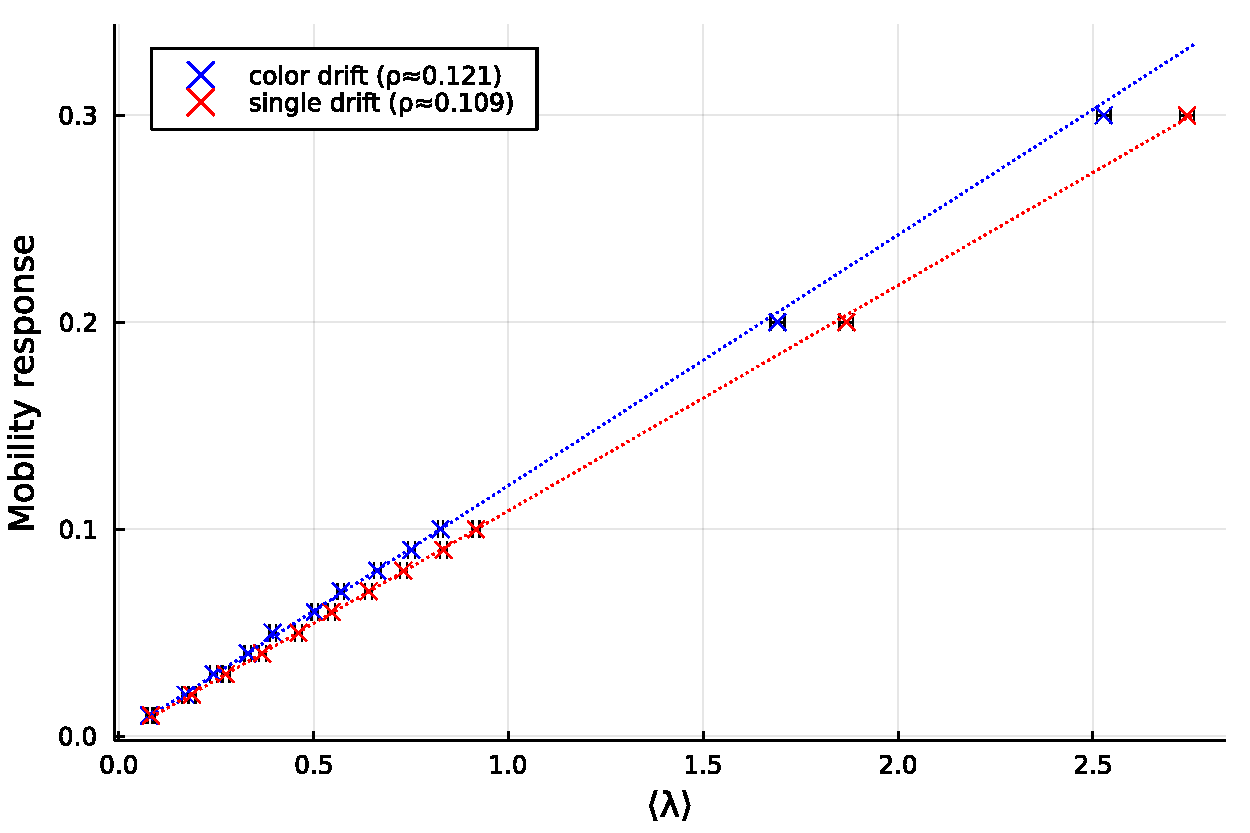
\includegraphics[width=0.9\linewidth]{figures/norton_mobility_plot.pdf}
      \caption{ \label{fig:norton_mobility_linear}
        Mobility response versus average forcing intensity in the linear regime. Least squares linear regression lines are plotted in dotted line, and the estimated transport coefficients are indicated in the legend.
      }
    \end{center}
  \end{figure}

  \begin{figure}[htbp]
    \begin{center}
      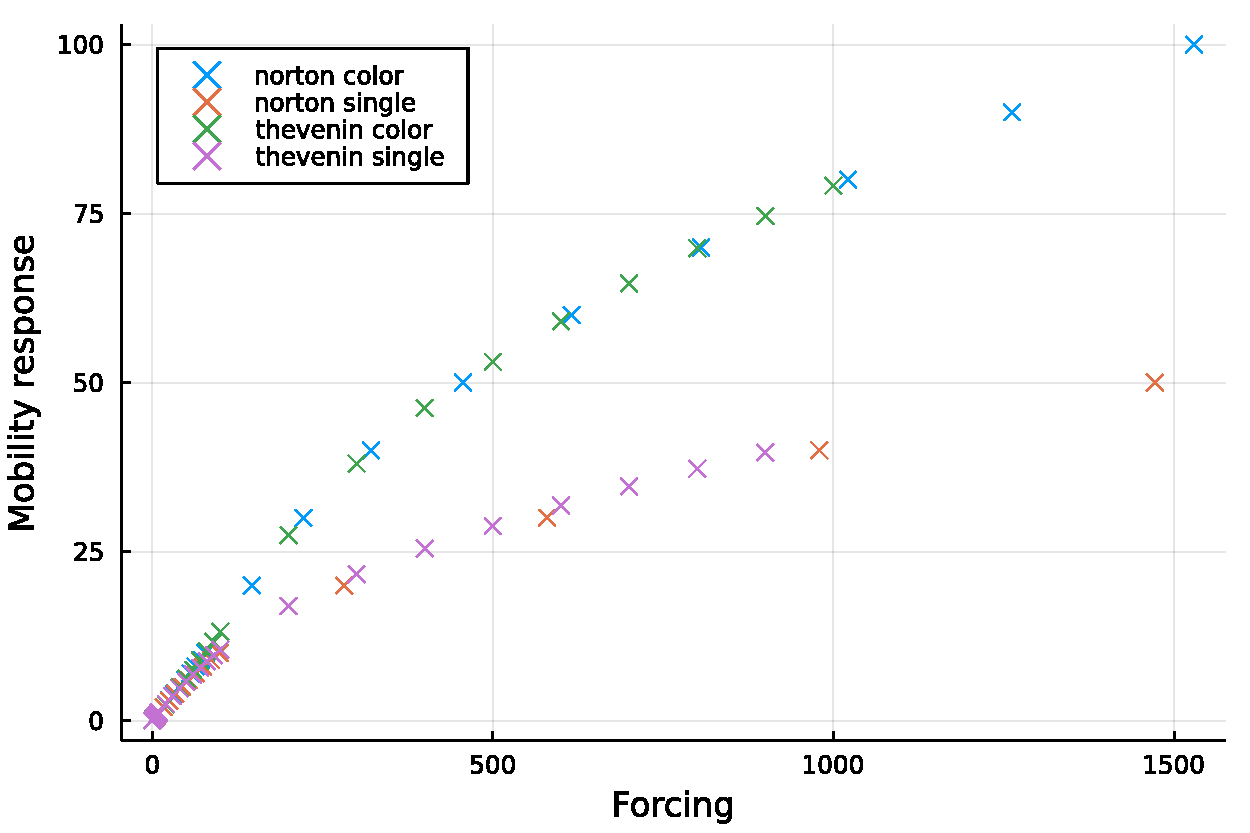
\includegraphics[width=0.7\linewidth]{figures/norton_mobility_full.pdf}
      \caption{ \label{fig:norton_mobility_full}
        Comparison of the Thévenin and Norton mobility equations of state.
      }
    \end{center}
  \end{figure}

  \begin{figure}[htbp]
    \begin{center}
      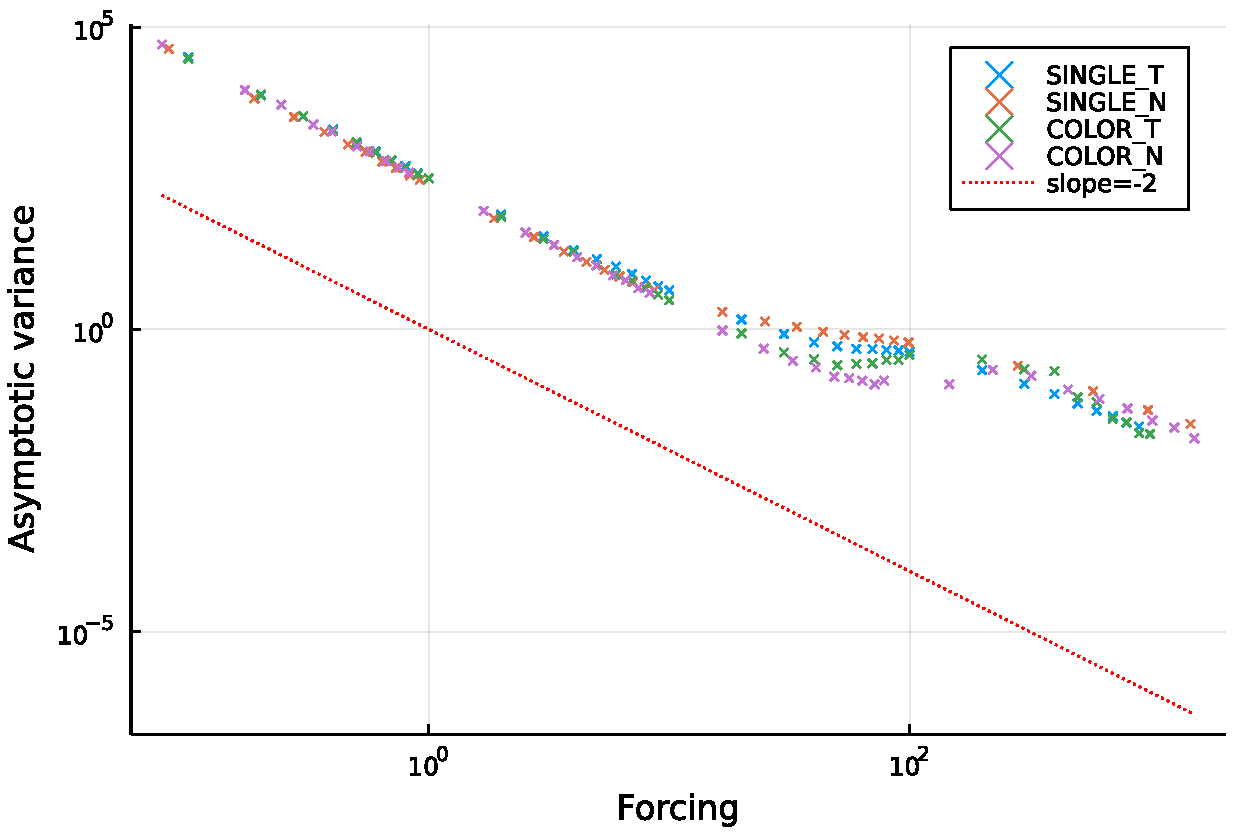
\includegraphics[width=0.7\linewidth]{figures/asymptotic_vars_mobility.pdf}
      \caption{ \label{fig:norton_avs}
       Plot of the asymptotic variance as a function of the forcing intensity for the different methods, on a log-log plot.
       Results corresponding to a Thévenin estimator are denoted with a T, and those corresponding to the Norton estimator are denoted with a N. 
      }
    \end{center}
  \end{figure}

\subsection{Shear viscosity}
The NEMD response observable \eqref{eq:nemd_shear_viscosity_response} for shear viscosity can be recovered in the form 
\[R_k(q,p)= \widetilde{G}_k(q)\cdot p\]
 by setting
\begin{equation}
    \label{eq:shear_viscosity_response_alt}
    \forall\, 1\leq i\leq N,\,\forall\, 2\leq \alpha\leq d,\qquad \widetilde{G}_k(q)_{i1}=\frac{1}{m}\exp\left(\frac{2ik\pi q_{i2}}{L}\right),\qquad \widetilde{G}_k(q)_{i\alpha}=0.
\end{equation}
Thus we can apply the Norton method. In practice, to avoid dealing with a complex exponential, we rather define
\begin{equation}
    \label{eq:shear_viscosity_response}
    \forall\, 1\leq i\leq N,\,\forall\, 2\leq \alpha\leq d,\qquad G_k(q)_{i1}=\frac{1}{m}\sin\left(\frac{2k\pi q_{i2}}{L}\right),\qquad G_k(q)_{i\alpha}=0.
\end{equation}
This can be achieved at no cost to generality by considering an appropriate translation of the forcing profile with respect to the results of Figure \ref{tab:fourier_coefficients}.
Estimators for the transport coefficient \eqref{eq:shear_viscosity_tranpsort_coefficient} and estimates of the statistical error can be obtained identically to the mobility case.
All simulations were run in the reference thermodynamics condition \eqref{eq:reference_thermo_condition_sv} for a minimum length of $8\times 10^7$ timesteps.

In Figure \ref{fig:norton_sv_linear_response}, we plot the normalized response \[\frac{R_1}{c_1(f_y)}\] against the estimated average forcing $\langle \lambda \rangle$ in the linear regime, for the different forcing profiles.
The estimated transport coefficients are consistent with one another, and agree with those obtained in the Thévenin and Green--Kubo setting.
In Figure \ref{fig:norton_sv_nonlinear_response}, we compare the non-linear response profiles between the Thévenin and Norton methods, for each of the forcing profiles. In every case, the responses coincide perfectly throughout.
In Figure \ref{fig:norton_avs_sv} we compare asymptotic variances of the finite difference estimators of the normalized response $\rho_{F,1}/c_1(f_y)$ using the Thévenin and Norton method. The asymptotic variance was estimated directly from the response time series in the Thévenin case, using a block averaging procedure,
and for the Norton method, a block averaging procedure on the forcing time series was combined with a delta-method. We find that the Norton estimators consistently outperform their Thévenin counterparts. Furthermore, it appears not all forcing profiles are equal in terms of asymptotic variance.
\begin{figure}[htbp]
  \begin{center}
    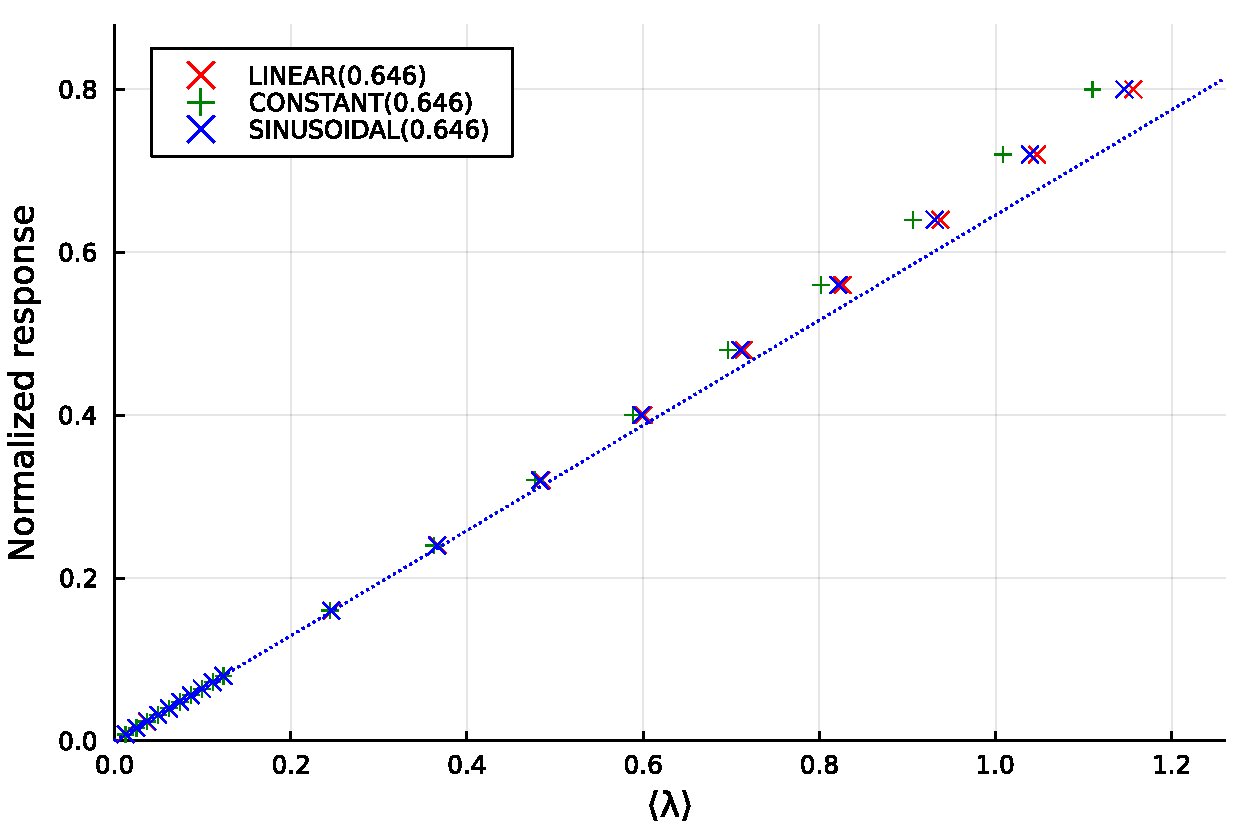
\includegraphics[width=0.9\linewidth]{figures/norton_sv_lin.pdf}
    \caption{ \label{fig:norton_sv_linear_response}
      Normalized Fourier response versus forcing intensity for the three transverse forcing profiles.
      The size of the linear response regime is roughly the same for every type of forcing. Least squares linear regression lines on the 10 first values are plotted in dotted line, and estimated normalized transport coefficients are indicated in the legend.
    }
  \end{center}
\end{figure}
\begin{figure}[htbp]
    \begin{center}
      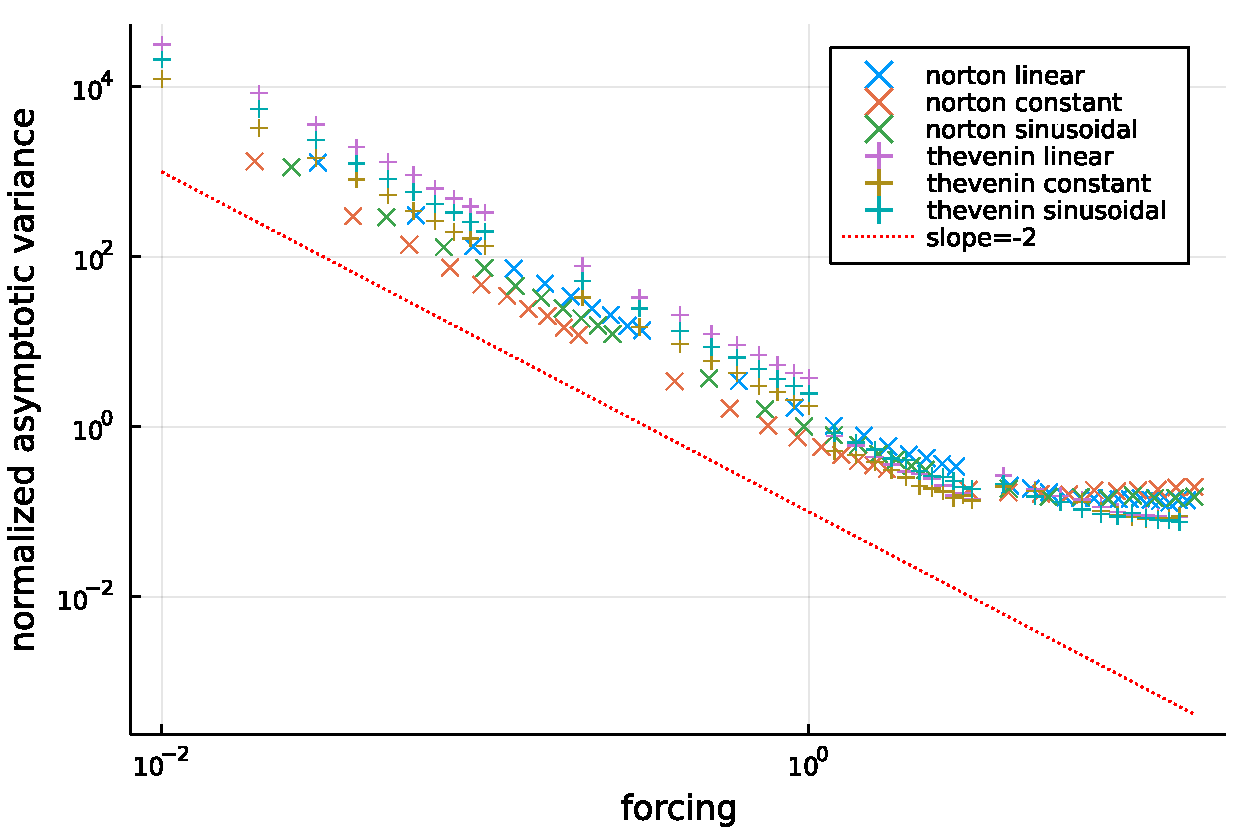
\includegraphics[width=0.9\linewidth]{figures/norton_sv_avs.pdf}
      \caption{ \label{fig:norton_avs_sv}
        Scaling of the asymptotic variance for the finite difference estimator of the normalized transport coefficient for shear viscosity}
    \end{center}
  \end{figure}

  \begin{figure}[htbp]
    \begin{center}
      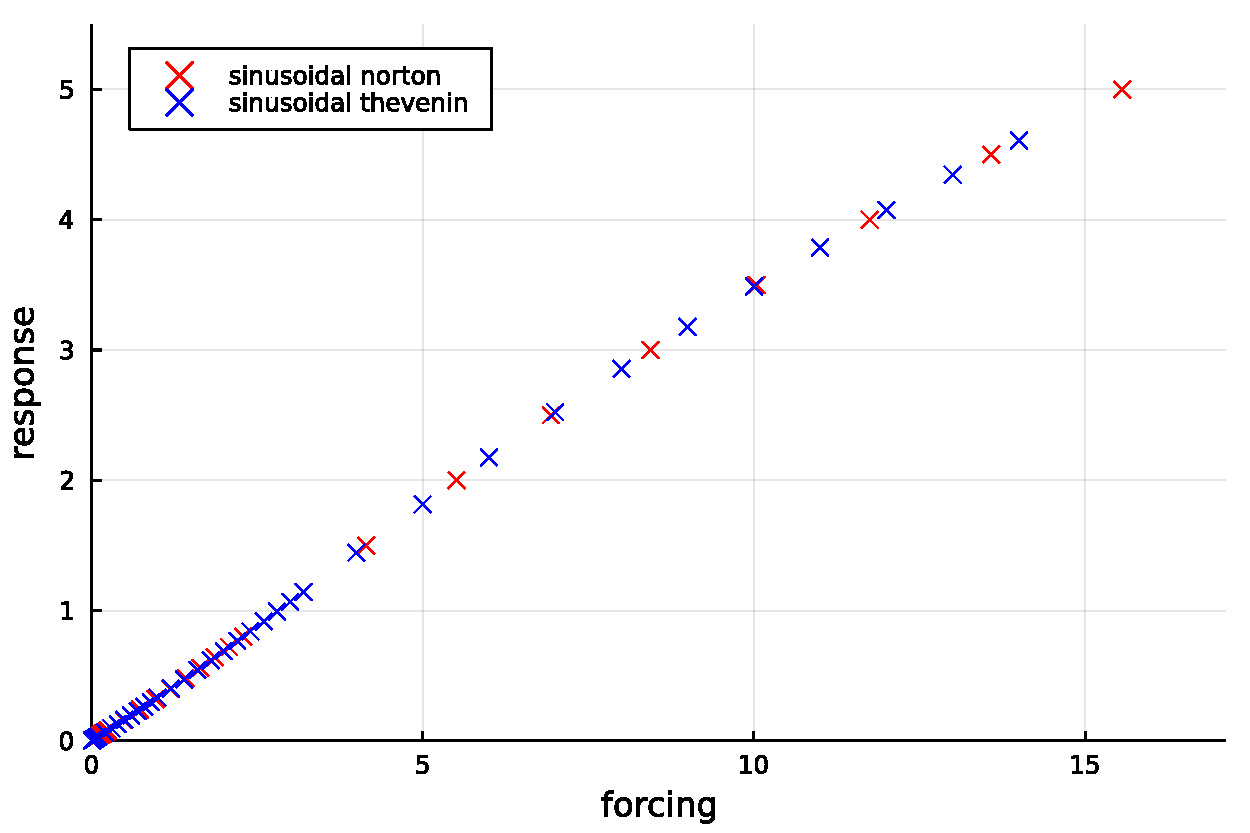
\includegraphics[width=0.75\linewidth]{figures/sinusoidal_joint.pdf}
      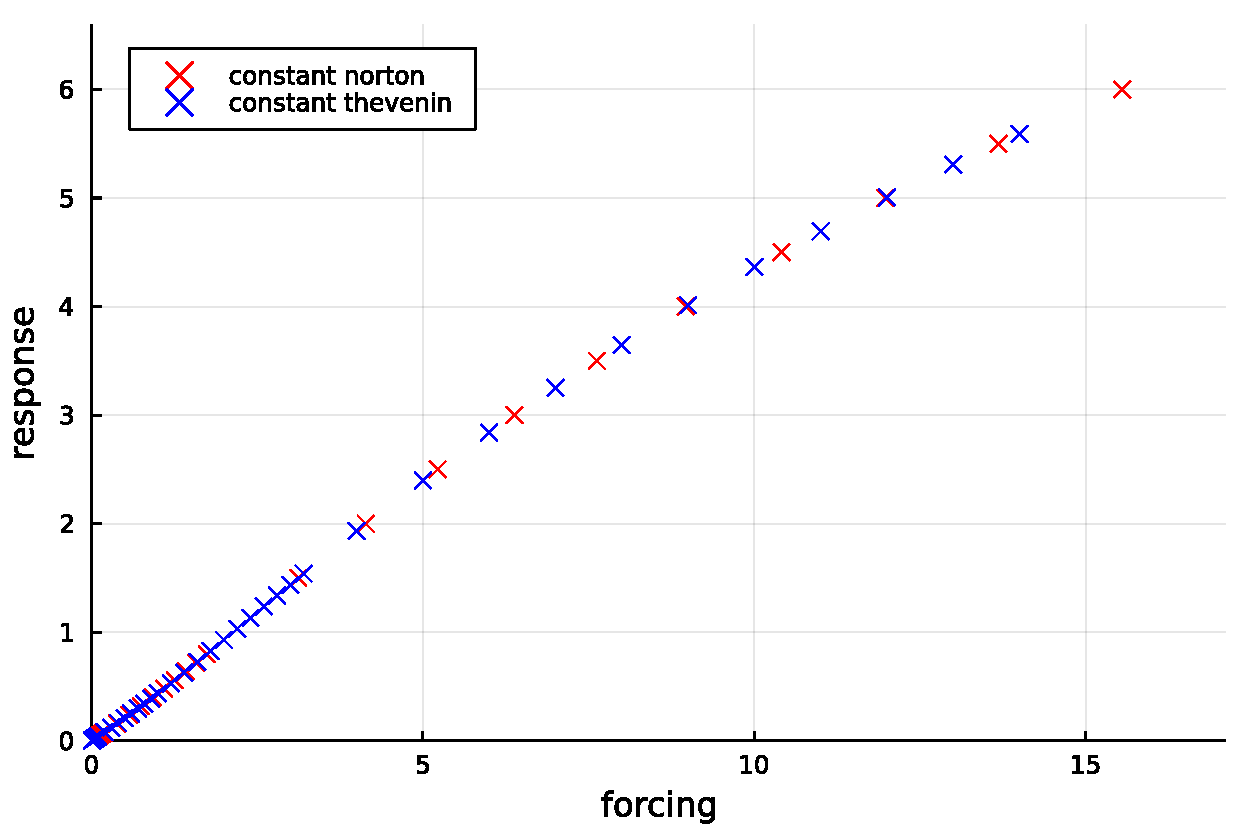
\includegraphics[width=0.75\linewidth]{figures/constant_joint.pdf}
      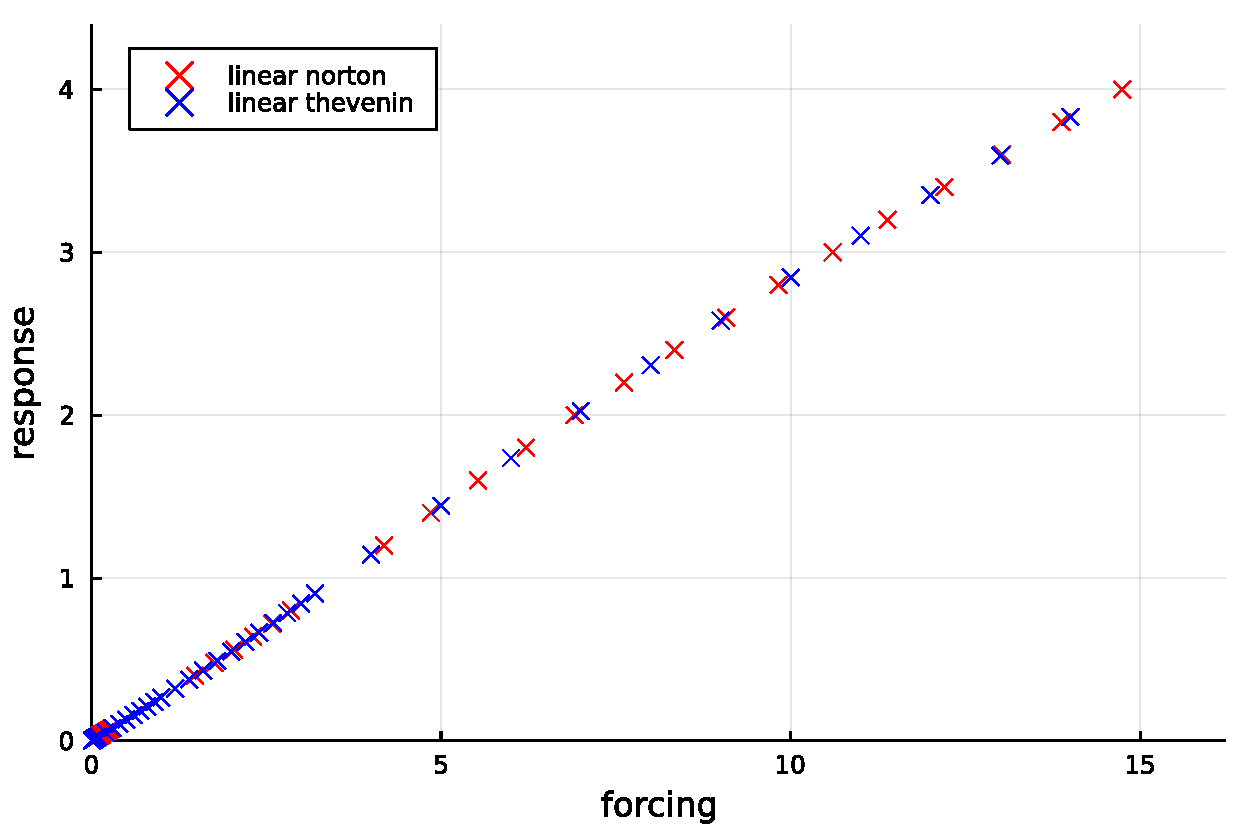
\includegraphics[width=0.75\linewidth]{figures/linear_joint.pdf}
      \caption{ \label{fig:norton_sv_nonlinear_response}
        Norton and Thévenin equations of state for the shear-viscosity Fourier response, for each type of forcing profile.
      }
    \end{center}
  \end{figure}
